\chapter{Thread Level Parallelism}
\label{c-tlp}

\section{Taxonomy}

Flynn
\begin{description}
    \item[SISD] Single Instruction Single Data (Modern uniprocessors)
    \item[SIMD] Single Instruction Multiple Data (Vector machines, and some multimedia)
    \item[MISD] Multiple Instruction Single Data (No commercial, possible in special applications)
    \item[MIMD] Multiple Instruction Multiple Data (Modern multiprocessors)
\end{description}


MIMD is broken into two groups based on memory configuration.  Memory is either shared equally by all processors or distributed among the processors.

\section{Shared Memory}

The first group centralizes the memory and has each processor with its cache connect via a shared memory bus.

\begin{figure}[h]
  % Requires \usepackage{graphicx}
  \begin{center}
  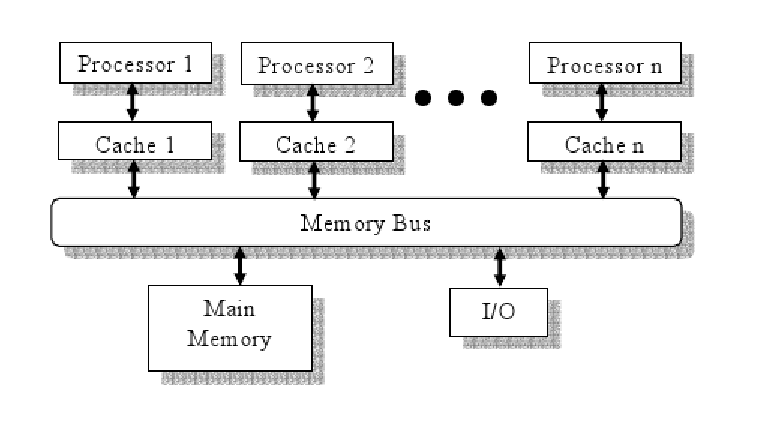
\includegraphics[width=4in]{smp.eps} \\
  \caption{Centralized shared memory multiprocessor}\label{f-smp}
  \end{center}
\end{figure}

The first group is also referred to by
\begin{itemize}
    \item Centralized Shared Memory
    \item Symmetric Multiprocessors (SMP)
    \item Uniform Memory Access (UMA)
\end{itemize}
These alternate titles are used since the the memory is central and shared, it is thus symmetric to all, and thus the access for each processor is uniform.  The main problem here is that as the number of processors grows, the need for memory bandwidth grows.  Without the needed bandwidth, requests will have to be scheduled resulting in increased latency.

\begin{example}
Using Figure 6.10 in the book, fill in the table, assuming all events are for an address relative to a cache in a SMP system.

\begin{tabular}{|l|l|l|} \hline
Event      & Source & State   \\ \hline
Startup    & -      & Invalid \\ \hline
Read Miss  & CPU    &         \\ \hline
Read Miss  & Bus    &         \\ \hline
Write Hit  & CPU    &         \\ \hline
Write Miss & Bus    &         \\ \hline
Write Miss & CPU    &         \\ \hline
Read Miss  & Bus    &         \\ \hline
\end{tabular}

{\color{ans}


\begin{tabular}{|l|l|l|} \hline
Event      & Source & State     \\ \hline
Startup    & -      & Invalid   \\ \hline
Read Miss  & CPU    & Shared    \\ \hline
Read Miss  & Bus    & Shared    \\ \hline
Write Hit  & CPU    & Exclusive \\ \hline
Write Miss & Bus    & Invalid   \\ \hline
Write Miss & CPU    & Exclusive \\ \hline
Read Miss  & Bus    & Shared    \\ \hline
\end{tabular}}
\end{example}

\section{Distributed Memory}

The second group distributes the memory to each processor so the memory bandwidth grows with the need.  This results in the problem of data sharing and communications between the nodes.
\begin{figure}[h]
  % Requires \usepackage{graphicx}
  \begin{center}
  \includegraphics[width=4in]{distributed.eps}\\
  \caption{Distributed memory multiprocessor}\label{f-distributed}
  \end{center}
\end{figure}
We could just treat the distributed memories like one big memory, giving each an address (shared address space).  This would allow the memories to be shared.  Access to different parts of memory is no longer uniform (addresses corresponding to ``local" memory will be fast and the addresses corresponding to ``remote" memory will be slow).  This scheme is referred to as
\begin{itemize}
    \item Distributed Shared Memory (DSM)
    \item Nonuniform Memory Access (NUMA)
\end{itemize}

Alternately we could keep each address space separate (local addresses) and pass messages between nodes containing the data or communications.  This scheme makes each machine look like an individual computer (multi-computers) and often each processor is a separate machine (clusters).

Shades of grey exist between the two, for instance a network OS can use message passing to pass a page of memory and implement what looks like shared address space by utilizing paging capabilities.


\section{Performance}

Amdahl's Law, for n processors is
\beq
S=\frac{1}{\sum_{i=1}^n\left(\frac{f_i}{i}\right)},
\eeq
where $f_i$ is the fraction of time when $i$ processors are busy.  Note that
\beq
\sum_{i=1}^nf_i=1.
\eeq

\begin{example}
Consider a 4 processor machine.  What must the fractions be to ensure a speedup of at least 3.

\beqn
3&=&\frac{1}{\frac{f_1}{1}+\frac{f_2}{2}+\frac{f_3}{3}+\frac{f_4}{4}} \\
1&=&3\left(\frac{f_1}{1}+\frac{f_2}{2}+\frac{f_3}{3}+\frac{f_4}{4}\right) \\
4&=&12f_1+6f_2+4f_3+3f_4
\eeqn
Note that if the least common multiple of the numbers $1$ through $n$ is denoted $LCM$, then for an $n$ processor system trying to achieve a speedup of $s$ we can say
\beqn
\frac{LCM}{s}=\sum_{i=1}^{n}\frac{LCM}{i}f_i
\eeqn
is the equation describing this situation that has integer coefficients.  We also know
\beqn
1&=&f_1+f_2+f_3+f_4.
\eeqn
Combining yields
\beqn
\bmat
4 \\
1
\emat
&=&
\bmat
12 & 6 & 4 & 3 \\
 1 & 1 & 1 & 1
\emat
\bmat
f_1 \\
f_2 \\
f_3 \\
f_4
\emat.
\eeqn
This is indefinite (more unknowns than equations), but we can solve for the fractions in terms of $f_1$ and $f_2$.
\beqn
8f_1+2f_2&=&f_4 \\
1-9f_1-3f_2&=&f_3
\eeqn
The second equation implies that individually $f_1<\frac{1}{9}\approx .11$ and $f_2<\frac{1}{3}\approx .33$ and together $3f_1+f_2\leq\frac{1}{3}$.  Further, if $f_3$ is negligible then $.67\leq f_4\leq .88$ is the minimum range to ensure a speedup of 3.
\end{example}

The last example shows how great the required thread level parallelism is to achieve a reasonable speedup.  The lack of thread level parallelism is one of the two great problems/challenges in multiprocessing.  The other great problem/challenge is the latency of remote accesses, which effectively adds a fixed penalty to the CPI of each processor thereby limiting performance.

The efficiency is given by
\beq
E &=& \sum_{i=1}^n\left(f_i\frac{i}{n}\right) \leq 1
\eeq

Scientific programs are often used to benchmark multiprocessor performance.  For the following table $n$ is the problem size, $p$ is the number of processors, and the $\alpha$ numbers are the scaling factors.

\vspace{.1in}
\begin{tabular}{lll}
Application & $\alpha_{compute}$  & $\alpha_{communicate}$ \\
FFT         & $\frac{n\log n}{p}$ & $\frac{n}{p}$ \\
LU/Ocean    & $\frac{n}{p}$       & $\sqrt{\frac{n}{p}}$ \\
Barnes-Hut  & $\frac{n\log n}{p}$ & $\sqrt{\frac{n}{p}}\log n$ \\
\end{tabular}
\vspace{.1in}

\begin{example}
An Ocean application takes 1 hour to run on a uniprocessor, and 33 minutes on a dual processor.  How long will it take to run the Ocean application on a problem 16 times the original size on a 128 processor machine?

{\color{ans}

\begin{tabular}{lcccc} \hline
Processors(p) & Size(n) & Time   & Computation        & Communication                    \\ \hline
1             & 1       & 1 hour & 1                  & 0                                \\ \hline
2             & 1       & 33 min & $\frac{1}{2}$       & $\frac{\sqrt{1}}{\sqrt{2}}$      \\ \hline
128           & 16      &        & $\frac{16}{128}$   & $\frac{\sqrt{16}}{\sqrt{128}}$   \\
              &         &        & $\frac{1}{8}$      & $\frac{1}{2\sqrt{2}}$            \\ \hline
\end{tabular}

From the table, if we call the base time of computation x, and the base time of communication y then we get (using minutes to be consistent):

\beq
60 &=& 1x+0y \\
33 &=& .5x+\frac{1}{\sqrt{2}}y
\eeq

from the first equation, $x=60 min$ and from the second equation $y=3\sqrt{2} min$. Thus the time for the third case (problem solution) is
\beqn
T &=& \frac{1}{8}x + \frac{1}{2\sqrt2}y \\
  &=& \frac{1}{8}60 + \frac{1}{2\sqrt2}3\sqrt{2} \\
  &=& 7.5 + 1.5 \\
  &=& 9 min
\eeqn
 }
\end{example}

\begin{example}
An LU application runs in 4000 seconds on a uniprocessor.  The same problem runs in 1020 seconds on a four processor machine.  How long will it take to run on a 16 processor machine?  How long will it take to run on a 64 processor machine?

\beqn
4000 &=& 1x+0y \\
1020 &=& .25x+.5y
\eeqn
So $x=4000$ and $y=40$.  Using this,
\beqn
\frac{1}{16}4000+\frac{1}{4}40&=& 250+10 \\
&=& 260
\eeqn
So a 16 processor machine runs it in 260 seconds.
\beqn
\frac{1}{64}4000+\frac{1}{8}40&=& 62.5+5 \\
&=& 67.5
\eeqn
Note that communication takes up $\frac{20}{1020}\approx .0196$ or just under 2\% of the time on a four processor.  When we have a sixteen processor machine it takes up $\frac{10}{260}\approx .0385$ or about 3.85\% of the time.  On the 64 processor machine the communication took up $\frac{5}{67.5}\approx .0385$ or about 7.41\% of the time.  Communication takes ever increasing fraction of the time, and becomes a limit to performance.  Consider running this on a 4096 processor machine.  It would take
\beqn
\frac{1}{4096}4000+\frac{1}{64}40&\approx& .977 + .625 \\
&\approx& 1.6
\eeqn
Thus communication takes $\frac{.625}{1.6}\approx .391$ or almost 40\% of the time!
\end{example} 